%(BEGIN_QUESTION)
% Copyright 2006, Tony R. Kuphaldt, released under the Creative Commons Attribution License (v 1.0)
% This means you may do almost anything with this work of mine, so long as you give me proper credit

Anta at vi har en tilstand der PV-signalet er 5.8 PSI og SP-signalet er 7.2 PSI. Bestem trykket i resetbelgen i det øyeblikket utgangssignalet er 11.3 PSI, og avgjør om utgangstrykket vil være {\it stigende} eller {\it fallende}:

$$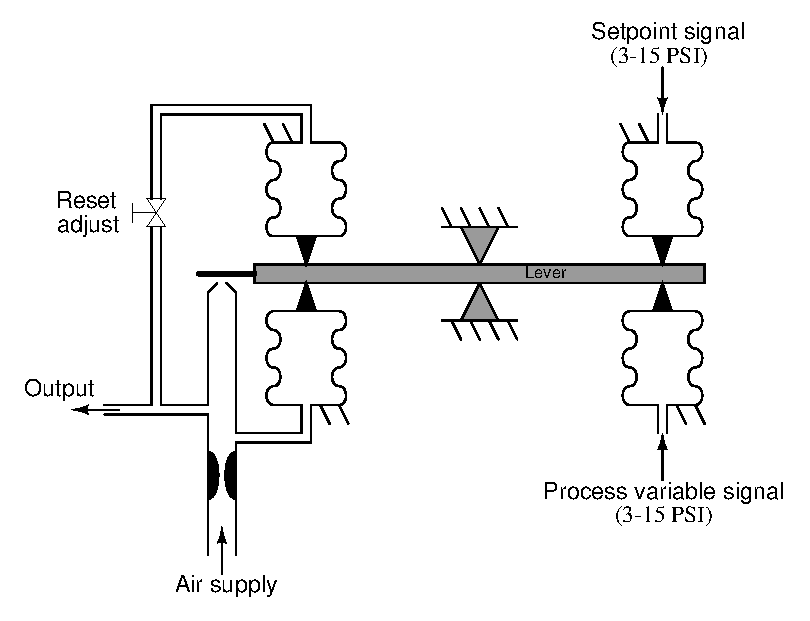
\includegraphics[width=15.5cm]{i01633x01.eps}$$

Anta at alle fire belgene er identiske i dimensjoner og konstruksjon, og at vippepunktet er plassert nøyaktig midt mellom de to belgsettene.

\vfil 

\underbar{file i01633}
\eject
%(END_QUESTION)





%(BEGIN_ANSWER)

Dette er et vurdert spørsmål -- ingen svar eller hint er gitt!

%(END_ANSWER)





%(BEGIN_NOTES)

Trykk i resetbelg = 12.7 PSI

\vskip 10pt

Utgangstrykket vil være {\it fallende} over tid.

\vskip 10pt

Et generelt prinsipp for alle kraftbalansemekanismer er at -- åpenbart -- alle krefter må være i balanse. Dersom setpunktsignalet er større enn PV-signalet (resulterende kraft {\it nedover} på høyre side av armen, som skaper et medurs moment), må trykket i resetbelgen være større enn trykket i utgangsbelgen (resulterende kraft {\it nedover} på armen, som skaper et moturs moment). Når alle belger har lik størrelse og lik avstand fra vippepunktet, kan vi konkludere med at ubalansen i signaltrykk på venstre side må være den samme som ubalansen i trykk på høyre side. Med SP 1.4 PSI høyere enn PV må trykket i resetbelgen også være 1.4 PSI høyere enn i utgangsbelgen, og dermed må trykket i resetbelgen være 12.7 PSI.

Når det gjelder retningen på trykkendringen i resetbelgen, kan vi bruke to helt ulike prinsipper og komme frem til samme resultat. Det ene prinsippet er at resetvirkningen skal ``winde'' i retning som passer regulatorens virkemåte. I dette tilfellet ser vi at regulatoren er direktevirkende, og derfor skal en tilstand der PV $<$ SP gi {\it avtakende} utgangstrykk, som betyr at trykket i resetbelgen også avtar. Et annet prinsipp er retningen på fluidstrøm gjennom en struping ved kjent trykkfall: resetjusteringsventilen har høyere trykk på oversiden (resetbelgsiden) enn på undersiden (utgangen), noe som forteller oss at luftstrømmen gjennom ventilen går nedover og tømmer luft fra resetbelgen (tenk på en motstand som leder konvensjonell strøm nedover fordi potensialet er høyere (+) på toppen enn på bunnen).

%INDEX% Control, proportional + integral: pneumatic force-balance controller

%(END_NOTES)
